\chapter{Referencial Teórico}
\label{cap:literature-review}
Como o objetivo desta pesquisa se concentra em investigar por meio de aprendizagem de máquina a documentação de projetos de software livre, a revisão bibliográfica foi dividida em quatro seções: Na Seção \ref{cap:free-software} é descrita uma breve explicação sobre o que é software livre, e como comunidades de desenvolvedores se organizam neste contexto. Na Seção \ref{cap:newcomers-barriers}, é introduzido o conceito de barreiras enfrentadas por novatos em software livre, e as implicações que tais barreiras geram em tais comunidades. Na Seção \ref{cap:documentation-problems} são apresentados problemas associados a documentação de projetos de software, dando ênfase aqueles em software livre.

% What is Open Source Software
% Why Open Source Software are important
% Who Maintains Open Source Software Active
% Difference between proprietary open source and proprietary software
% Joining Process of Open Source Communities (Define/discuss newcomers in FLOSS)

\section{Software Livre}

\label{cap:free-software}
Software livre (do inglês, \textit{free software}) é o software que em sua essência é distribuído livremente, geralmente acompanhado por uma licença de software livre, e que conta com a disponibilização de seu código-fonte em algum meio acessível a usuários e desenvolvedores \citet{Gacek:2004:MMO:968720.968793}. Um programa de computador para ser considerado livre deve fornecer a quem o utiliza quatro liberdades essenciais \citep{stallman2002free}:
\begin{itemize}
    \item A liberdade de executar o programa, para qualquer propósito;
    \item A liberdade de estudar como o programa funciona, e poder adaptá-lo a qualquer necessidade (Acesso ao código fonte é uma precondição a esta liberdade);
    \item A liberdade de redistribuir cópias do programa a outros usuários;
    \item A liberdade de aperfeiçoar o programa, e poder liberar os aperfeiçoamentos, de modo com que toda a comunidade se beneficie das mudanças feitas (Acesso ao código fonte também é uma precondição a esta liberdade).
\end{itemize}
Outro termo geralmente associado a software livre é o conceito de software de código aberto (do inglês, \textit{open source software}). Apesar das diferenças\footnote{\url{https://www.gnu.org/philosophy/open-source-misses-the-point.html}} entre software livre e de código aberto, nesta pesquisa consideramos os termos como sinônimos. Um possível antônimo para software livre é o software proprietário, que restringe legalmente a terceiros o acesso ao código fonte do programa desenvolvido~\citep{fuggetta2003open}.

O modo como programas de software livre são construídos pode variar. Geralmente, um novo projeto de software livre se inicia quando algum programador possui uma ideia, problema ou porção de código a ser desenvolvido. O desenvolvedor submete sua proposta à comunidades colaborativas anunciando sua ideia a outros desenvolvedores, onde estes, quando atraídos pelo projeto, se unem ao grupo de desenvolvedores \citep{raymond1999cathedral}. Com o tempo, o número de contribuidores tende a crescer, e uma nova comunidade passa a se formar em torno do projeto. Para prosseguir com o desenvolvimento, plataformas de codificação passam a ser utilizadas como meio de gerenciamento do código fonte, e canais de comunicação são estabelecidos entre os membros da comunidade. 

O desenvolvimento de projetos de software livre usualmente ocorre de maneira colaborativa \citep{von2003community}. As contribuições são usualmente voluntárias, o que significa que desenvolvedores não são remunerados financeiramente por suas contribuições \citep{osterloh2007open}.

% Descrever melhor o processo de contribuição (Talvez com uma imagem)

Em termos de organização, as definições variam de acordo com a literatura \citep{nakakoji2002evolution, jergensen2011onion}. \citet{crowston2005social}, por exemplo, sintetizam a estrutura social  de um projeto de software livre a partir de um modelo de camadas. Segundo os autores, na camada mais interna se encontram os principais desenvolvedores, aqueles que geralmente contribuem com a maior parte do código fonte e são responsáveis por revisar futuras contribuições. Ao meio da estrutura se encontram os co-desenvolvedores, membros do projeto que são responsáveis por contribuir com correções e aprimoramentos. E por fim, nas duas camadas exteriores, se encontram os usuários ativos, que não contribuem com o código fonte mas usualmente relatam problemas, e os usuários passivos, que apenas desfrutam dos recursos oferecidos. A representação deste modelo de camadas é apresentada na Figura \ref{fig:onion-model}.  % Usar uma referência que use novatos

\begin{figure}
    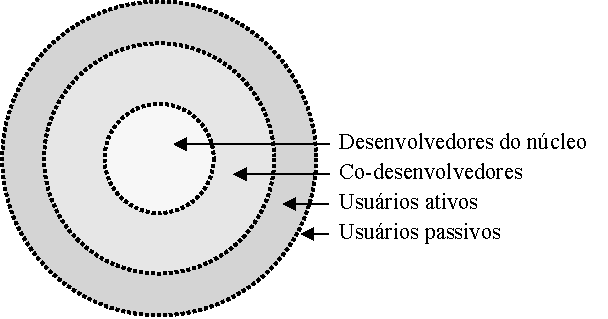
\includegraphics[width=0.65\textwidth]{figuras/onion_model.pdf}
    \caption{Estrutura em camadas de uma comunidade de software livre.}
    \label{fig:onion-model}
\end{figure}

Pra contribuir com um projeto de software livre, um desenvolvedor adquire uma cópia do código fonte do projeto através de uma plataforma de codificação, implementa modificações, e submete as mudanças novamente ao repositório oficial do projeto~\citep{mockus2000case}. As mudanças são revisadas por um grupo de mantenedores e, quando de acordo com os critérios de aceitação, são anexadas aos binários do programa.

Além dos grupos apresentados pelo modelo de \citet{crowston2005social}, existem ainda os novos contribuidores que, apesar de não necessariamente constituírem parte da hierarquia de um projeto, são amplamente estudados pela literatura em software livre. Neste contexto, um novo contribuidor, novato ou recém-chegado, pode ser definido como um desenvolvedor interessado em ingressar em uma comunidade de software livre por meio de contribuições ao código fonte do projeto
\citep{nakakoji2002evolution}. Entre as razões pelas quais novatos são amplamente estudados pela literatura, se encontram as dificuldades que estes enfrentam ao tentarem ingressar em um projeto de software livre, como mostra a seção a seguir.

\section{Barreiras enfrentadas por novatos}
\label{cap:newcomers-barriers}
% Discuss Barriers in OSS
% Mention Igor Steinmacher and the categories he defined for newcomers barriers in OSS
Como as contribuições em software livre são em sua essência voluntárias, o ato de atrair novos contribuidores para tais comunidades é considerado fator essencial para continuidade de muitos projetos \citep{qureshi2011socialization}. Como em qualquer comunidade, se membros ao saírem de uma comunidade não forem repostos por novos contribuidores, a comunidade irá eventualmente deixar de existir, já que novatos podem ser considerados fonte de inovação, ideias e trabalho em tais comunidades \citep{kraut2012challenges}. 

No entanto, atrair novos contribuidores para uma comunidade de software livre não é uma tarefa trivial \citep{zhou2015whowill}. Em um estudo sobre empresas que compartilham comunidades neste contexto, \citet{dahlander2008how} mostram que até mesmo para comunidades bem estabelecidas como o MySQL, diversos problemas são enfrentados ao atrair novos contribuidores. Entre os problemas que justificam a baixa adesão de novatos, estão barreiras enfrentadas por estes durante a entrada nos projetos de software livre. 

\citet{von2003community} descrevem tais barreiras como um conjunto de dificuldades, empecilhos ou deficiências no processo de contribuição, que impossibilitam  desenvolvedores a realizar suas primeiras colaborações com projetos de software livre. De acordo com os autores, as barreiras estão intrinsecamente relacionadas ao nível de especialização de cada desenvolvedor. Como a complexidade de um software tende a crescer conforme seu desenvolvimento, ingressar durante em meio a execução do projeto tende a ser um processo lento e dificultoso a novos desenvolvedores que, por muitas vezes, desconhecem os processos e tecnologias utilizadas pela comunidade.

\citet{hannebauer2017relationship} dividem barreiras enfrentadas por novatos em duas categorias, submissão e modificação. De acordo com os autores, novatos tendem a enfrentar dificuldades tanto durante a elaboração de uma nova contribuição, como durante o processo de submissão do código modificado ao projeto. Em uma perspectiva complementar, \citet{steinmacher@thehard} mostram que tais barreiras não somente estão associadas as motivações e características do desenvolvedor ao contribuir com um projeto, como também são desencadeadas por problemas da própria comunidade a qual ele almeja participar. Problemas como falta de documentação e a má recepção fornecida a novos contribuidores, são exemplos de problemas que podem impactar a entrada dos novatos em tais comunidades.

Entre os estudos que se destacam ao identificar barreiras enfrentadas por novatos em software livre, se encontra o modelo proposto por \citet{steinmacher@preliminary}. Dividido em seis categorias diferentes, o modelo apresenta cinquenta e oito barreiras identificadas através de uma revisão sistemática da literatura, e de entrevistas com novos e experientes contribuidores em projetos de software livre. Entre as categorias, foram constatadas dificuldades relacionadas ao processo de recepção dos novatos nos projetos, características individuais dos novatos, falta de orientação durante o processo de contribuição, problemas com documentação, diferenças culturais e obstáculos técnicos.

O fato de tais comunidades não atraírem novos contribuidores o suficiente, usualmente implica na falta de condições necessárias para se manter o desenvolvimento dos projetos ativo, levando, por consequência, muitas comunidades de software livre a inatividade.

\section{Problemas em documentações de software}
\label{cap:documentation-problems}
% Talk about lack of documentation and how they affect the joining of newcomers in OSS

\section{Trabalhos Relacionados}
\label{cap:related-work}
\subsection{Apoio a novatos em software livre}
           Assumindo a necessidade de um processo sólido de retenção de novatos em projetos de software livre, uma diversidade de trabalhos relacionados são propostos para dar suporte a novos contribuidores em software livre. 

A seguir, apresentamos a Tabela , que descreve um conjunto de trabalhos relacionados que auxiliam novatos e projetos de software livre neste cenário:

\subsection{Classificação de documentações de software}

\section{Considerações finais}